\documentclass[12pt,a4paper,spanish$  $]{book}
\usepackage{xltxtra}
\usepackage{emptypage}
\usepackage[left=2cm,right=2cm,top=2cm,bottom=2cm]{geometry}
%\usepackage[top=1cm,bottom=1cm,left=0.5cm,right=0.5cm,asymmetric]{geometry}
\setlength\headheight{13.6pt}% as suggested by fancyhdr
%\usepackage{mwe}% only for dummy text and example pdf page
\usepackage{pdfpages}
\usepackage{fancyhdr}
\usepackage[spanish]{babel}
\usepackage[utf8]{inputenc}
\usepackage{multicol}
\usepackage{lilyglyphs}
\usepackage{subfiles}
\usepackage{hanging}
\usepackage[dayofweek]{datetime}    %yyyymmdd
\usepackage{lyluatex}
\usepackage{hyperref}

\usepackage[pages=some]{background}
\usepackage{microtype}	
\usepackage{setspace}

\setmainfont[Mapping=tex-text, Numbers={OldStyle}, Ligatures={Common}]{Linux Biolinum O}
\fontspec[Numbers={OldStyle}]{Linux Biolinum O}

\fancypagestyle{pdfpages}{
		\fancyhf{} 
		\renewcommand{\headrulewidth}{0pt} 
		\fancyfoot[LE]{\oldstylenums\thepage -- \oldstylenums\leftmark} %even page - chapter title
		\fancyfoot[RO]{\oldstylenums\rightmark -- \oldstylenums\thepage} %uneven page - section title
		
		\renewcommand{\dateseparator}{}
		\fancyfoot[LO]{\scriptsize\the\year\twodigit{\the\month}\twodigit{\the\day}}
		\fancyfoot[RE]{\scriptsize\the\year\twodigit{\the\month}\twodigit{\the\day}} 
}

\newcommand*\pdfpagesheaderleft{}
\newcommand*\pdfpagesheadercenter{}
\newcommand*\pdfpagesheaderright{}

\newcommand{\setlayout}[3]{\thispagestyle{pdfpages}%
  \gdef\pdfpagesheaderleft{#1}%
  \gdef\pdfpagesheadercenter{#2}%
  \gdef\pdfpagesheaderright{#3}%
}

\hypersetup{
	colorlinks=true,
	linkcolor=blue,
	filecolor=magenta,      
	urlcolor=gray,
}

\backgroundsetup{contents=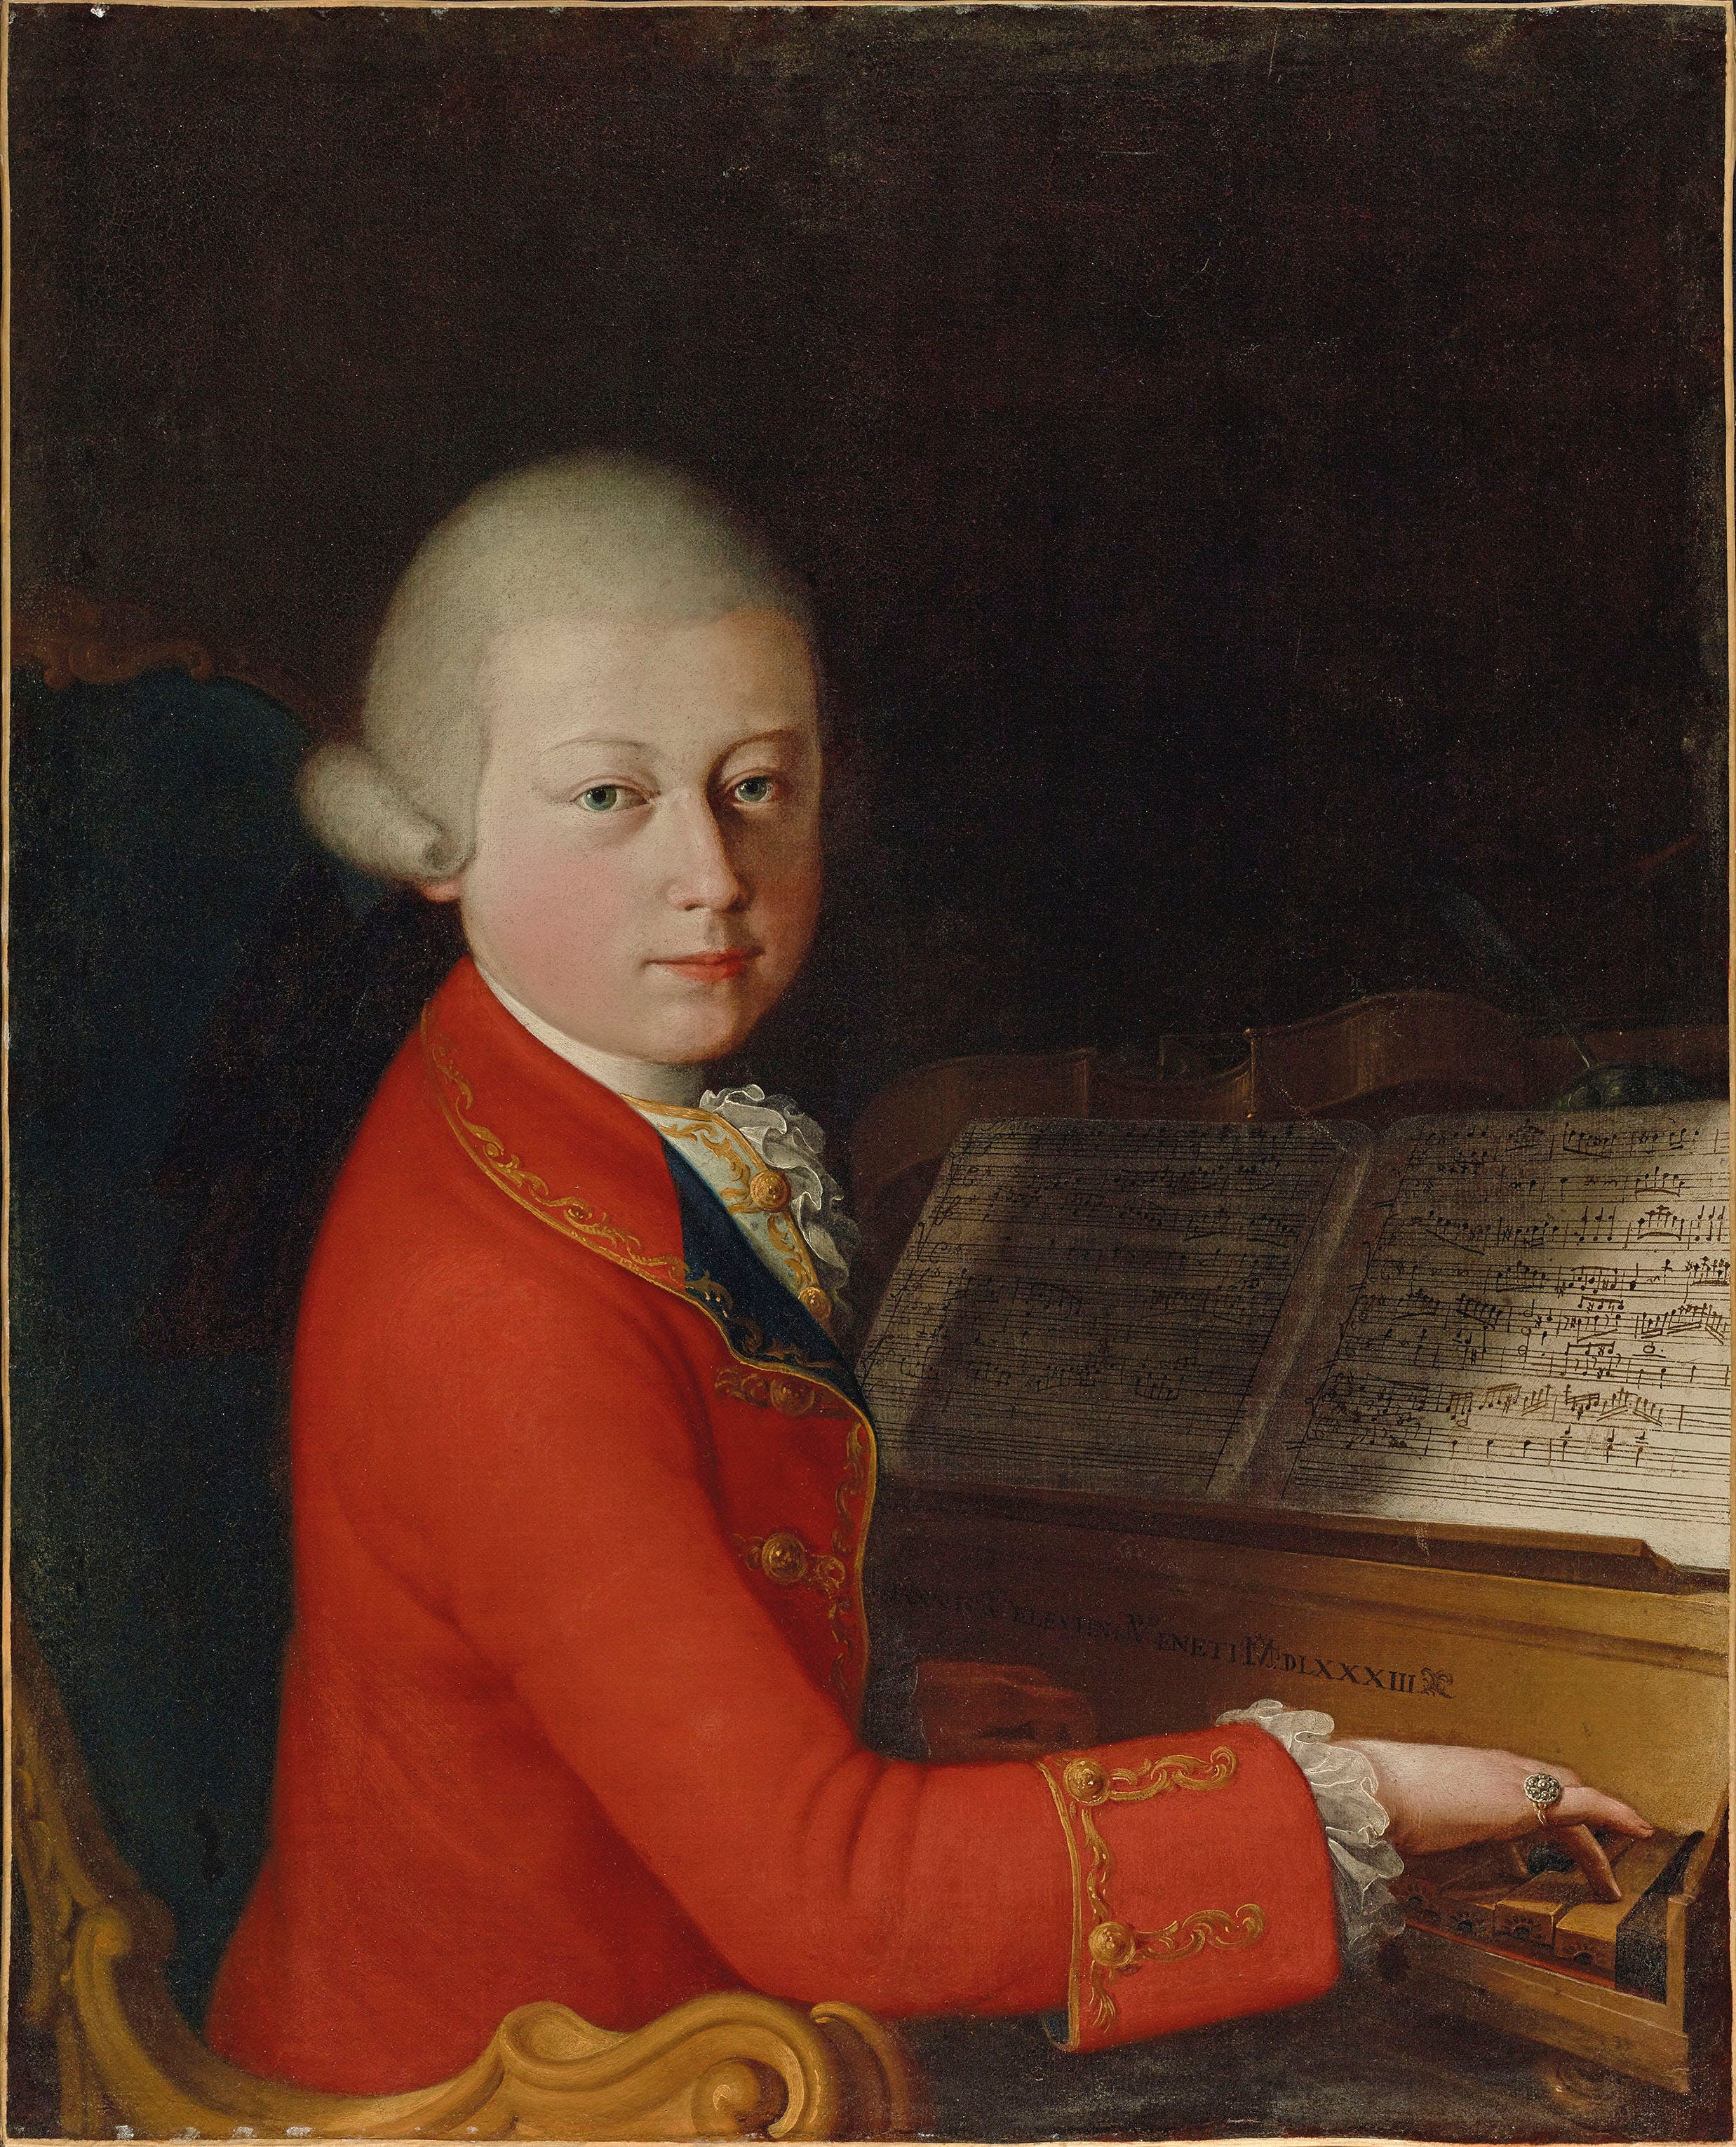
\includegraphics{./img/front.jpg},scale=0.5, opacity=0.2}

\begin{document}
		\frontmatter
		\begin{titlepage}
			\vspace*{4cm}
			\begin{flushright}
				\fontsize{100pt}{0pt}\selectfont \textls[-70]{w.a.mozart}
			\end{flushright}
			\vspace*{8cm}
			\begin{flushright}
				\fontsize{40pt}{50pt}\selectfont \textls*[-40]{serenata, ex C.}\\
				\fontsize{30pt}{20pt}\selectfont \textls*[-40]{k. 648}\\
				\fontsize{20pt}{20pt}\selectfont \textls*[-40]{a critical--practical edition} /
				\textls*[-40]{score and parts}\\
				\fontsize{20pt}{20pt}\selectfont \textls*[-40]{una edición crítico--práctica} /
				\textls*[-40]{partitura y partes}

			\end{flushright}
			\vfill
			\centering{\textsc{v.\the\year\twodigit{\the\month}\twodigit{\the\day}}\par}
			\BgThispage
			\newpage
		\end{titlepage}
		
		\cleardoublepage
		\pagestyle{empty}

		\setlength{\columnsep}{1cm}
		\onehalfspacing
		\begin{multicols}{2}
			\section*{Preface}
			In September 2024 the Internationale Stiftung Mozarteum Salzburg, together with musicologist Neal Zaslaw, presented the ninth edition of the catalog of Mozart's works, originally published by Ludwig von Köchel in 1862. In this edition the catalog goes up to number 721, bypassing the fateful «626» for the first time and thus abandoning the chronological criterion sought in previous editions. For the most part, these new «Koechel numbers» are pieces that were previously listed within the catalog's many appendices, but some are works recently attributed to the composer. 

This edition presents one of them, a «Serenade, ex C» for string trio (two violins, \emph{primo} and \emph{secondo}, plus a bass ---labeled as \emph{violoncello} in the \emph{particella} and as \emph{basso} on the title page) to which the number K. 648 has been assigned. This is a rather unusual work, presumably dating from the late 1760s. A copy of the \emph{particelle} is included in the collection of the German composer Carl Ferdinand Becker (1804-1877) and was digitized by the Leipziger Städtischen Bibliotheken in 2018. In September 2024, in conjunction with the publication of the new catalog edition, the piece was also performed again, presumably for the first time since it was written. 

This edition of the work is naturally based on this single copy. It is a critical--practical edition in the sense that, although all readings other than the manuscript are indicated graphically (using square brackets and dashed lines for the slurs), the aim is to ensure that these do not distract performers when performing the piece. We do not include an appendix detailing the readings adopted: the curious reader can simply consult the manuscript (available at http://digital.slub-dresden.de/id454516029) and draw his or her own conclusions. We also sought to respect some idiosyncrasies of the writing: the occasional «voice» writing in the string parts and the lack of markings of tuplets. Others, on the other hand, were not taken into account: the «kneed beams» (for instance, we replace 
    \begin{lilypond}[insert=inline,voffset=-1.5em]
        \relative c'{ \omit Score.Clef  \omit Score.TimeSignature \stemUp \tweak Beam.positions #'(-1 . -1) c8 \stemDown c' \stemUp c, \stemDown c'}
    \end{lilypond} 
    with 
    \begin{lilypond}[insert=inline, voffset=-1em]
        \relative c'{ \omit Score.Clef  \omit Score.TimeSignature c8 c'  c,  c'}
    \end{lilypond}
), the number of bars per system, and some stem directions. We believe that some of these particularities of the notation possess illocutionary force and convey intentions to performers. 

This edition is presented as an open edition: it was made entirely using Lilypond and Lua\LaTeX\ and its source code is available in an open repository on GitHub (https://github.com/fsarud/mozart648). Any corrections or changes can be made using that source code and recompiled to obtain the print version; also, if desired, those changes can be suggested for inclusion in the edition via a pull request. The music typography work was done by Luca Mariano and Federico Sarudiansky (fsarud at gmail dot com), who was also in charge of the final edition. 

Buenos Aires, September 2024.

			\section*{Prefacio}
			En septiembre de 2024 la Internationale Stiftung Mozarteum de Salzburgo, junto al musicólogo Neal Zaslaw presentaron la novena edición del catálogo de obras de Mozart, originalmente publicado por Ludwig von Köchel en 1862. En esta edición del catálogo llega hasta el número 721, traspasando por primera vez el fatídico «626» y abandonando así el criterio cronológico que se buscaba en las ediciones anteriores. En su mayor parte, estos nuevos «números Koechel» son piezas que antes figuraban dentro de los muchos anexos del catálogo, pero algunas son obras recientemente atribuidas al compositor. 

Esta edición presenta una de ellas, una «Serenata, ex C» para trío de cuerdas (dos violines, \emph{primo} y \emph{secondo}, más un bajo ---indicado como \emph{violoncello} en la \emph{particella} y como \emph{basso} en la carátula) al que le fue asignado el número K. 648. Se trata de una obra inusual, datada presumiblemente en los años finales de la década de 1760. Una copia de las \emph{particelle} de esta obra está incluida en la colección del compositor alemán Carl Ferdinand Becker (1804—1877) y fue digitalizada por la Leipziger Städtischen Bibliotheken en 2018. En septiembre de 2024, junto con la publicación de la nueva edición del catálogo, también se volvió a ejecutar la pieza, presumiblemente por primera vez desde que fue escrita. 

Esta edición de la obra se basa, naturalmente, en esta única copia. Se trata de una edición crítico—práctica en el sentido que, si bien se indican gráficamente todas las lecturas distintas al manuscrito (utilizando corchetes rectos y líneas punteadas para las ligaduras), se busca que estas no distraigan a los intérpretes a la hora de ejecutar la pieza. No incluimos un anexo detallando las lecturas adoptadas: el lector curioso simplemente puede consultar el manuscrito (disponible en \href{http://digital.slub-dresden.de/id454516029}{http://digital.slub-dresden.de/id454516029}) y extraer sus propias conclusiones. También buscamos respetar algunas idiosincrasias de la escritura: la ocasional escritura a voces en las partes de cuerdas y la falta de marcas de tresillos. Otras, en cambio, no fueron tenidas en cuenta: las «barras al medio» en los grupos de corcheas (por ejemplo, reemplazamos
    \begin{lilypond}[insert=inline,voffset=-1.5em]
        \relative c'{ \omit Score.Clef  \omit Score.TimeSignature \stemUp \tweak Beam.positions #'(-1 . -1) c8 \stemDown c' \stemUp c, \stemDown c'}
    \end{lilypond} 
    con 
    \begin{lilypond}[insert=inline, voffset=-1em]
        \relative c'{ \omit Score.Clef  \omit Score.TimeSignature c8 c'  c,  c'}
    \end{lilypond}
), la cantidad de compases por sistema, y algunas direcciones de plicas. Creemos que algunas de estas particularidades de la notación poseen fuerza ilocucionaria y transmiten intenciones a los intérpretes. 

Esta edición se presenta como una edición abierta: fue realizada íntegramente utilizando Lilypond y Lua\LaTeX\ y su código fuente se encuentra disponible en un repositorio abierto en GitHub (\href{https://github.com/fsarud/mozart648}{https://github.com/fsarud/mozart648}). Cualquier corrección o cambio puede hacerse utilizando ese código fuente y recompilarse para obtener la versión para imprimir; también, si se desea, se pueden sugerir esos cambios para su inclusión en la edición mediante un \emph{pull request}. El trabajo de tipografía musical fue realizado por Luca Mariano y Federico Sarudiansky (fsarud at gmail dot com), quien también tuvo a cargo la edición final. 

Buenos Aires, septiembre de 2024.


		\end{multicols}

		\mainmatter
		\renewcommand{\leftmark}{Serenata, ex C., K. 648--- Partitura}
		\renewcommand{\rightmark}{W. A. Mozart}
		\includepdf[pages=-, scale=0.97,pagecommand=\setlayout{}{Center}{Right corner} ]{./moz648-Score.pdf} 
		
		\mainmatter
		\renewcommand{\leftmark}{Serenata, ex C., K. 648--- Violino primo}
		\renewcommand{\rightmark}{W. A. Mozart}
		\includepdf[pages=-, scale=0.97,pagecommand=\setlayout{}{Center}{Right corner} ]{./moz648-vl1.pdf} 
		\cleardoublepage

		\mainmatter
		\renewcommand{\leftmark}{Serenata, ex C., K. 648--- Violino secondo}
		\renewcommand{\rightmark}{W. A. Mozart}
		\hspace{0pt} \vfill \noindent \fbox {This page is intentionally left blank} \\ \fbox {Esta página se deja intencionalmente en blanco} \vfill \hspace{0pt} \newpage
		\includepdf[pages=-, scale=0.97,pagecommand=\setlayout{}{Center}{Right corner} ]{./moz648-vl2.pdf} 
		\cleardoublepage

		\mainmatter
		\renewcommand{\leftmark}{Serenata, ex C., K. 648--- Basso/Violoncello}
		\renewcommand{\rightmark}{W. A. Mozart}
		\hspace{0pt} \vfill \noindent \fbox {This page is intentionally left blank} \\ \fbox {Esta página se deja intencionalmente en blanco} \vfill \hspace{0pt} \newpage
		\includepdf[pages=-, scale=0.97,pagecommand=\setlayout{}{Center}{Right corner} ]{./moz648-bc.pdf} 
		\cleardoublepage

% 		\mainmatter
% 		\renewcommand{\rightmark}{Luigi Boccherini- Sonata G. 2- Violoncello solo}
% 		\hspace{0pt} \vfill \fbox {Esta página se deja intencionalmente en blanco} \vfill \hspace{0pt} \newpage
% 		\renewcommand{\leftmark}{Sonata G. 2- Violoncello solo}
% 		\renewcommand{\rightmark}{Luigi Boccherini}
% 		\includepdf[pages=-, scale=0.97,pagecommand=\setlayout{}{Center}{Right corner} ]{song2-VcI.pdf} 
		
% 		\mainmatter
% %		\renewcommand{\rightmark}{Luigi Boccherini- Sonata G. 2- Violoncello secondo}
% %		\hspace{0pt} \vfill \fbox {Esta página se deja intencionalmente en blanco} \vfill \hspace{0pt} \newpage
% 		\renewcommand{\leftmark}{Sonata G. 2- \textit{Basso}}
% 		\renewcommand{\rightmark}{Luigi Boccherini}
% 		\includepdf[pages=-, scale=0.97,pagecommand=\setlayout{}{Center}{Right corner} ]{song2-VcII.pdf} 
		
\end{document}